%% Use the hmcposter class with the thesis document-class option.
\documentclass[thesis]{hmcposter}
\usepackage{graphicx}
\usepackage{natbib}
\usepackage{booktabs}
\usepackage{subfig}
\usepackage{amsmath}
\usepackage{textcomp}
\usepackage{url}
\usepackage{enumitem}
\setlist{leftmargin=2cm, labelsep=0.7cm}

%% Author of the thesis.
\author{Stetson Bost}

%% The year of your thesis poster's creation.
\posteryear{2017}

%% Thesis Title.
\title{Adaptive Nested Algorithms\\for Balanced Scheduling}

%% Advisor name.
\advisor{Weiqing Gu}

%% Define the \BibTeX command, used in our example document.
\providecommand{\bibtex}{{\rmfamily B\kern-.05em%
    \textsc{i\kern-.025em b}\kern-.08em%
    T\kern-.1667em\lower.7ex\hbox{E}\kern-.125emX}}


\pagestyle{fancy}

\begin{document}

\begin{poster}

\section{Introduction}
Scheduling is very important for maintaining order, for both individuals and larger organizations.
In a fast-paced environment like Harvey Mudd, schedules can help many people stay organized and manage stress.
With this project, we wanted to develop algorithms capable of creating effective and adaptable schedules.

\section{Algorithm for Personal Scheduling}%
Our algorithm for creating a personal schedule aims to both accomplish all necessary tasks and maintain a balanced lifestyle.
We treat a schedule as a collection of relatively short \emph{time slots}, and contiguous time slots can form \emph{blocks}.
A group of consecutive blocks can form a \emph{section}, identified by it starting block and ending block.
%TODO Explain what a task is (time slots, due dates, priority)
The algorithm has three nested components.
\begin{enumerate}
	\item
		Assign tasks to sections.
	\item
		Assign tasks to blocks within sections. 
	\item
		Assign tasks to time slots within blocks.
\end{enumerate}
Each of these steps takes into account various aspects of the tasks, including deadlines or available time windows, amount of time needed, and intensity. Additionally, each block has a minimum permissible amount of time reserved for non-work activities, which may or may not be structured, depending on user preference.
With this non-work time and by maintaining as equal intensity levels as possible among blocks, this algorithm prioritizes a balanced schedule.
%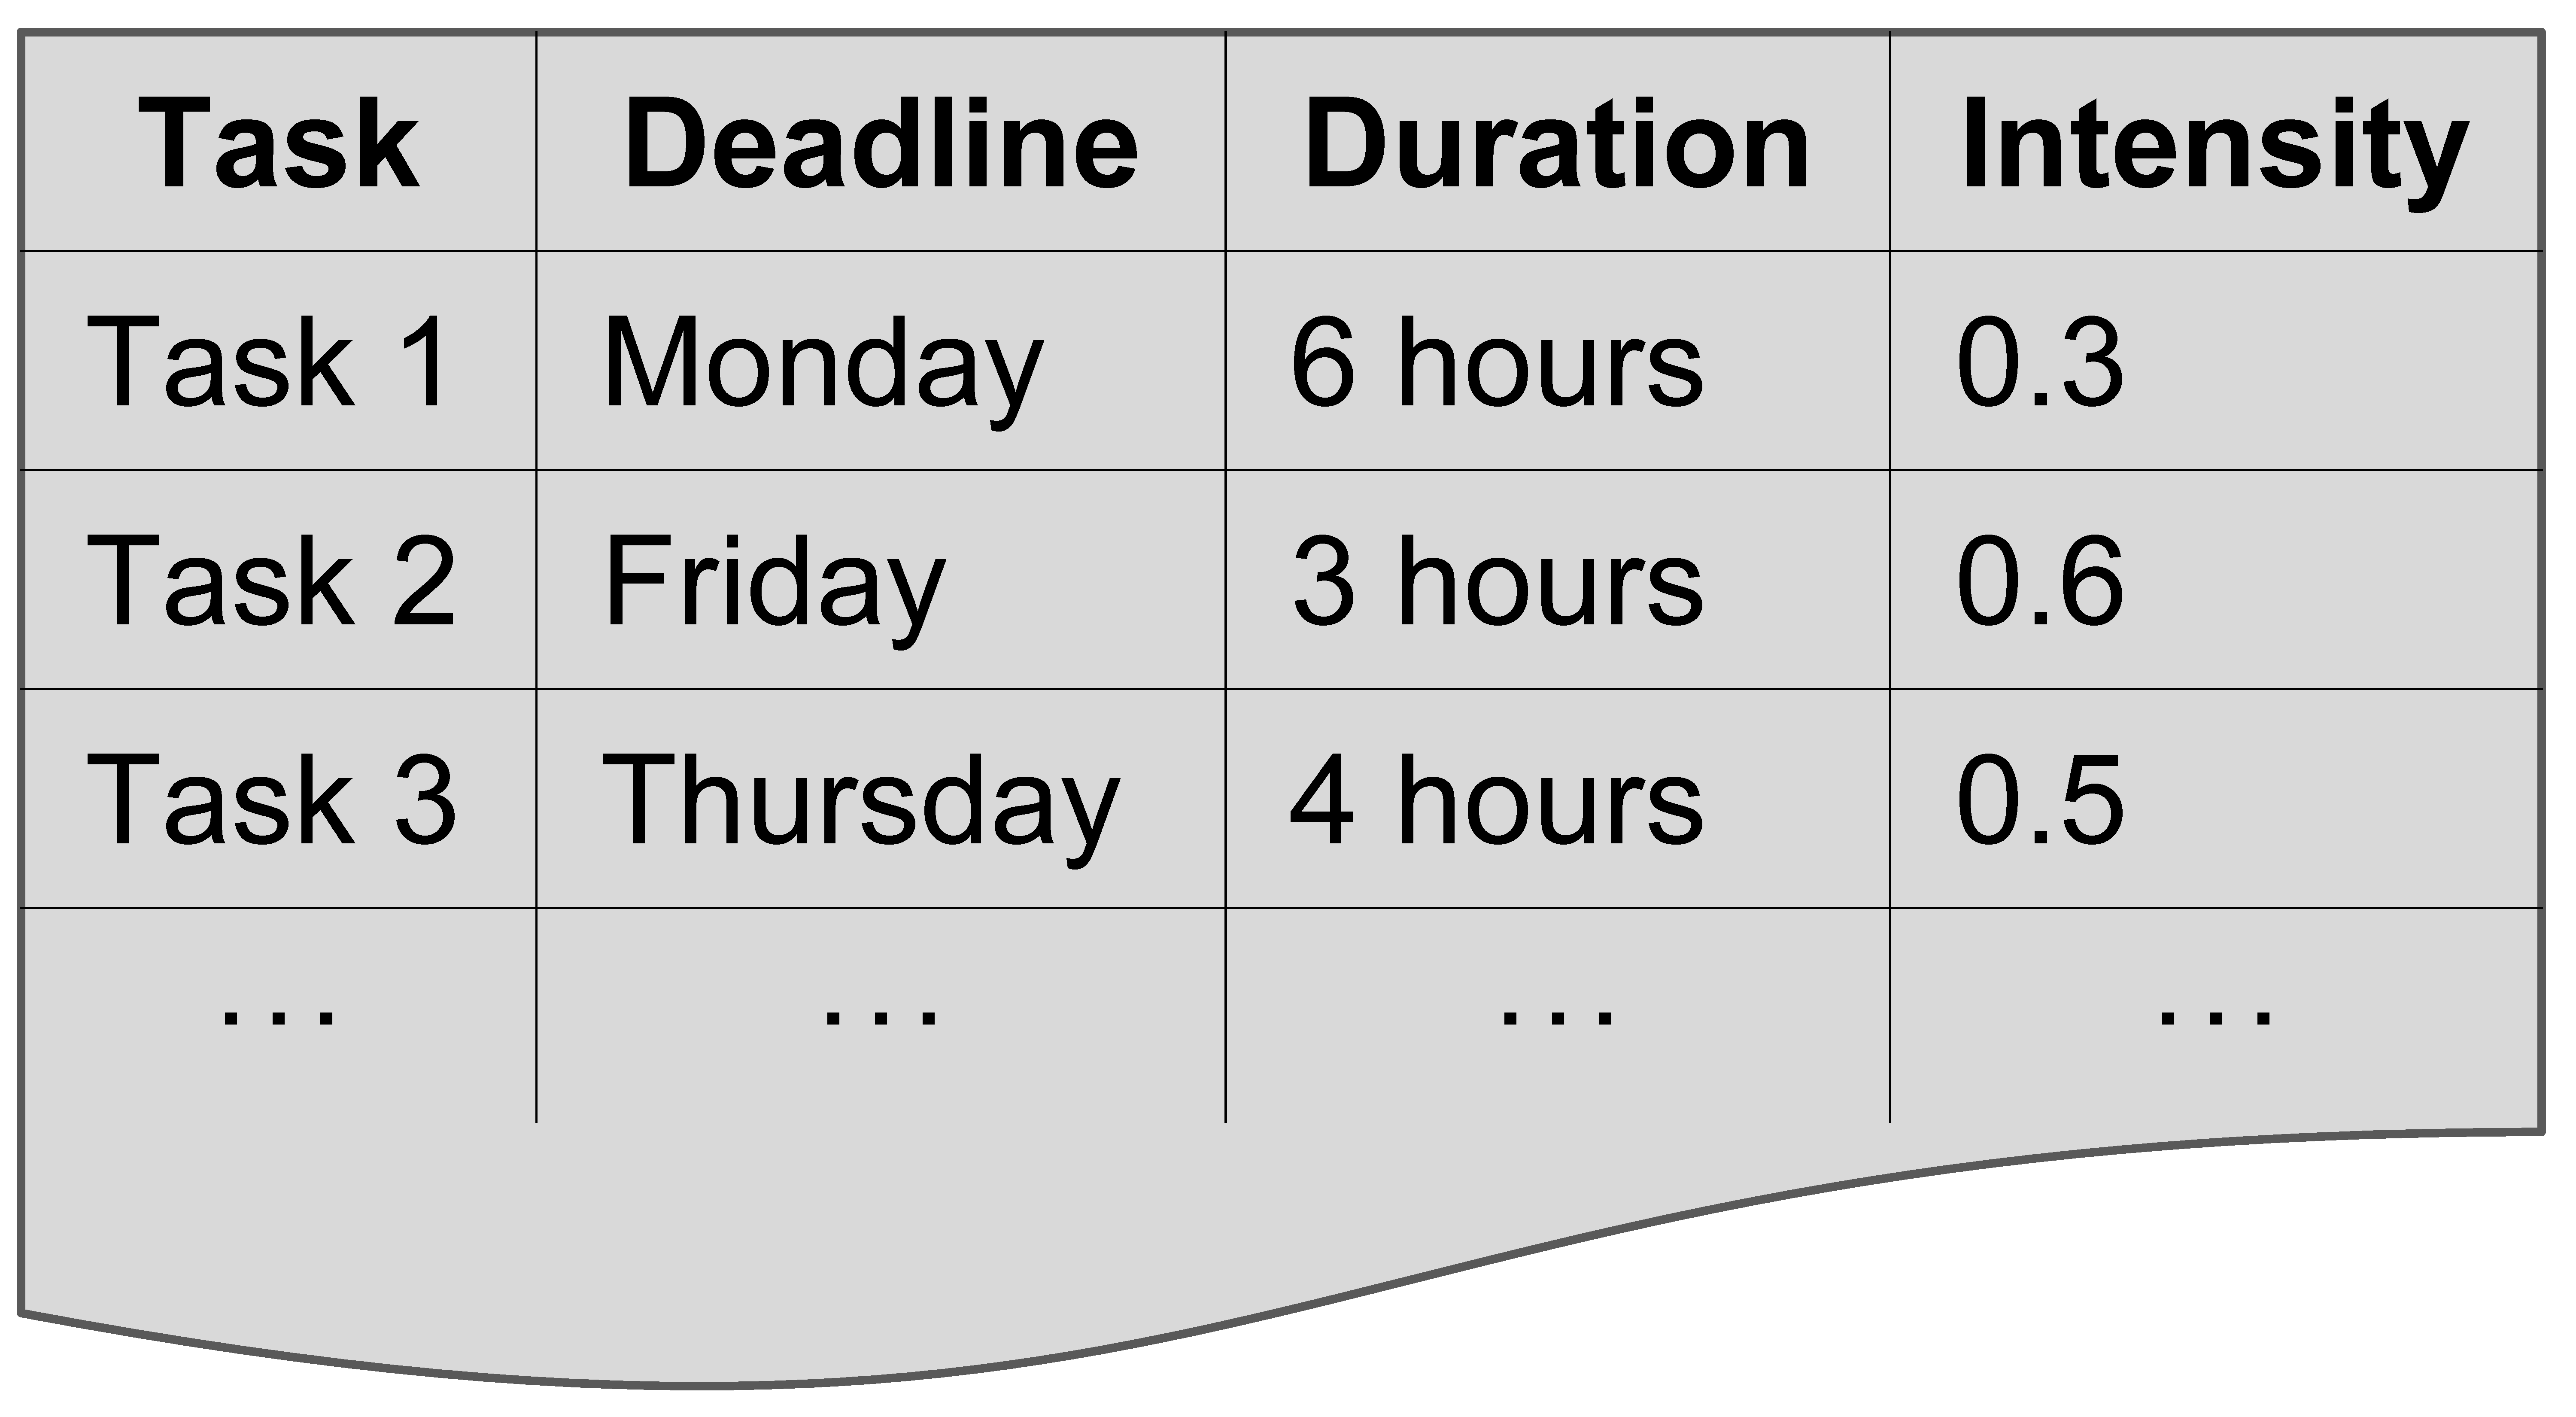
\includegraphics[scale=0.18]{TaskList.pdf}
%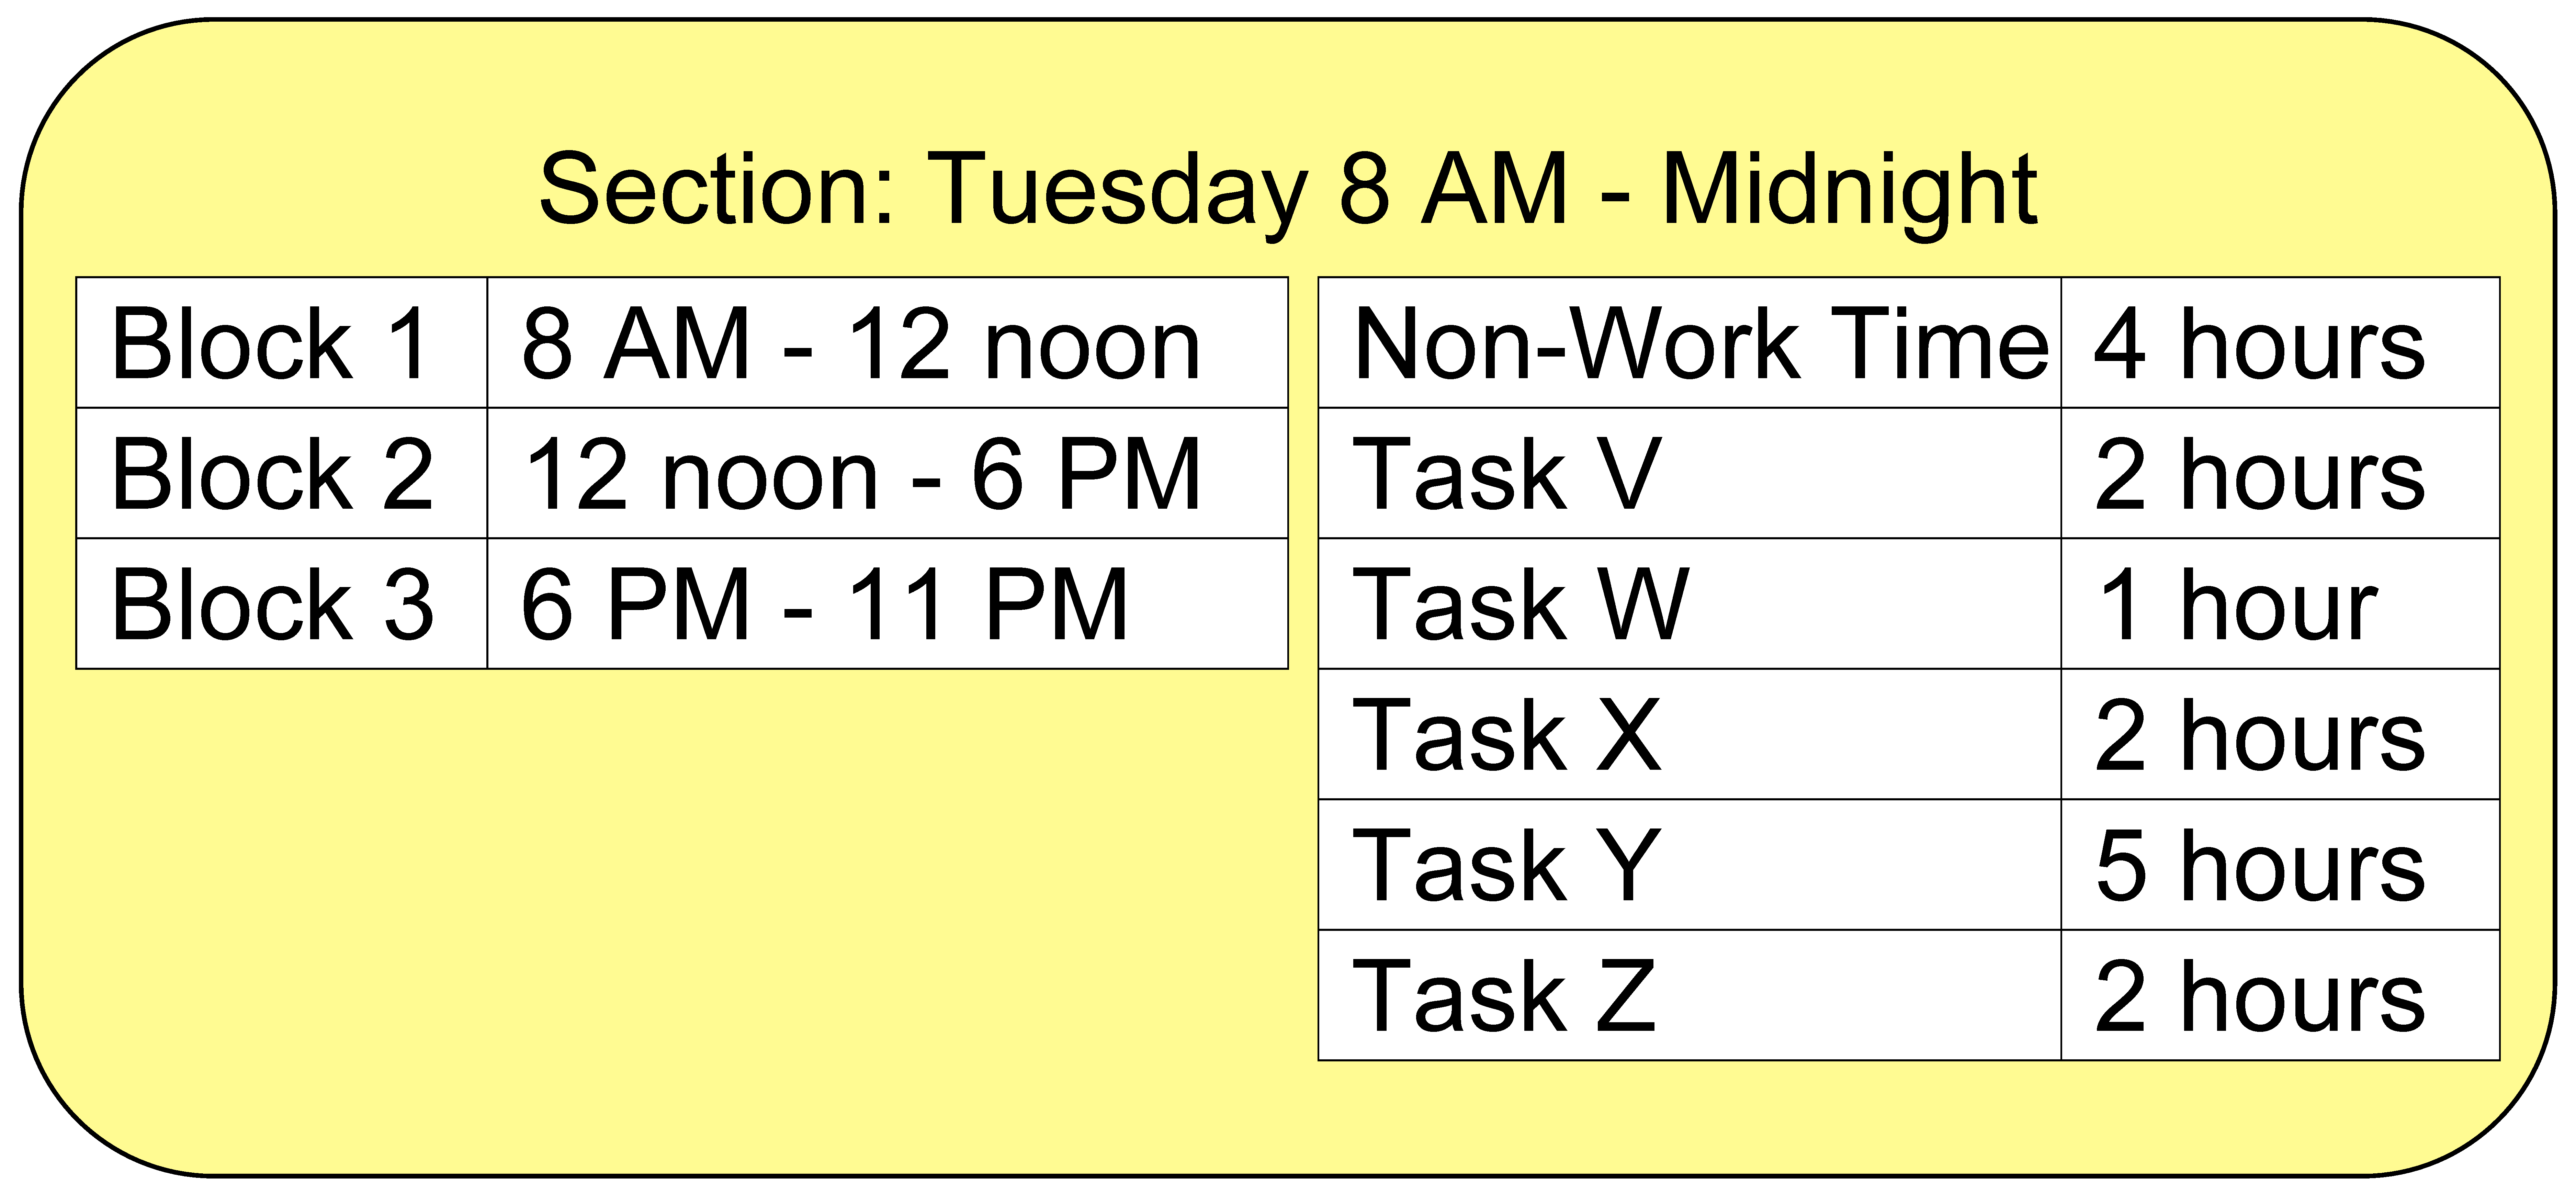
\includegraphics[width=0.48\columnwidth]{Section.pdf}
%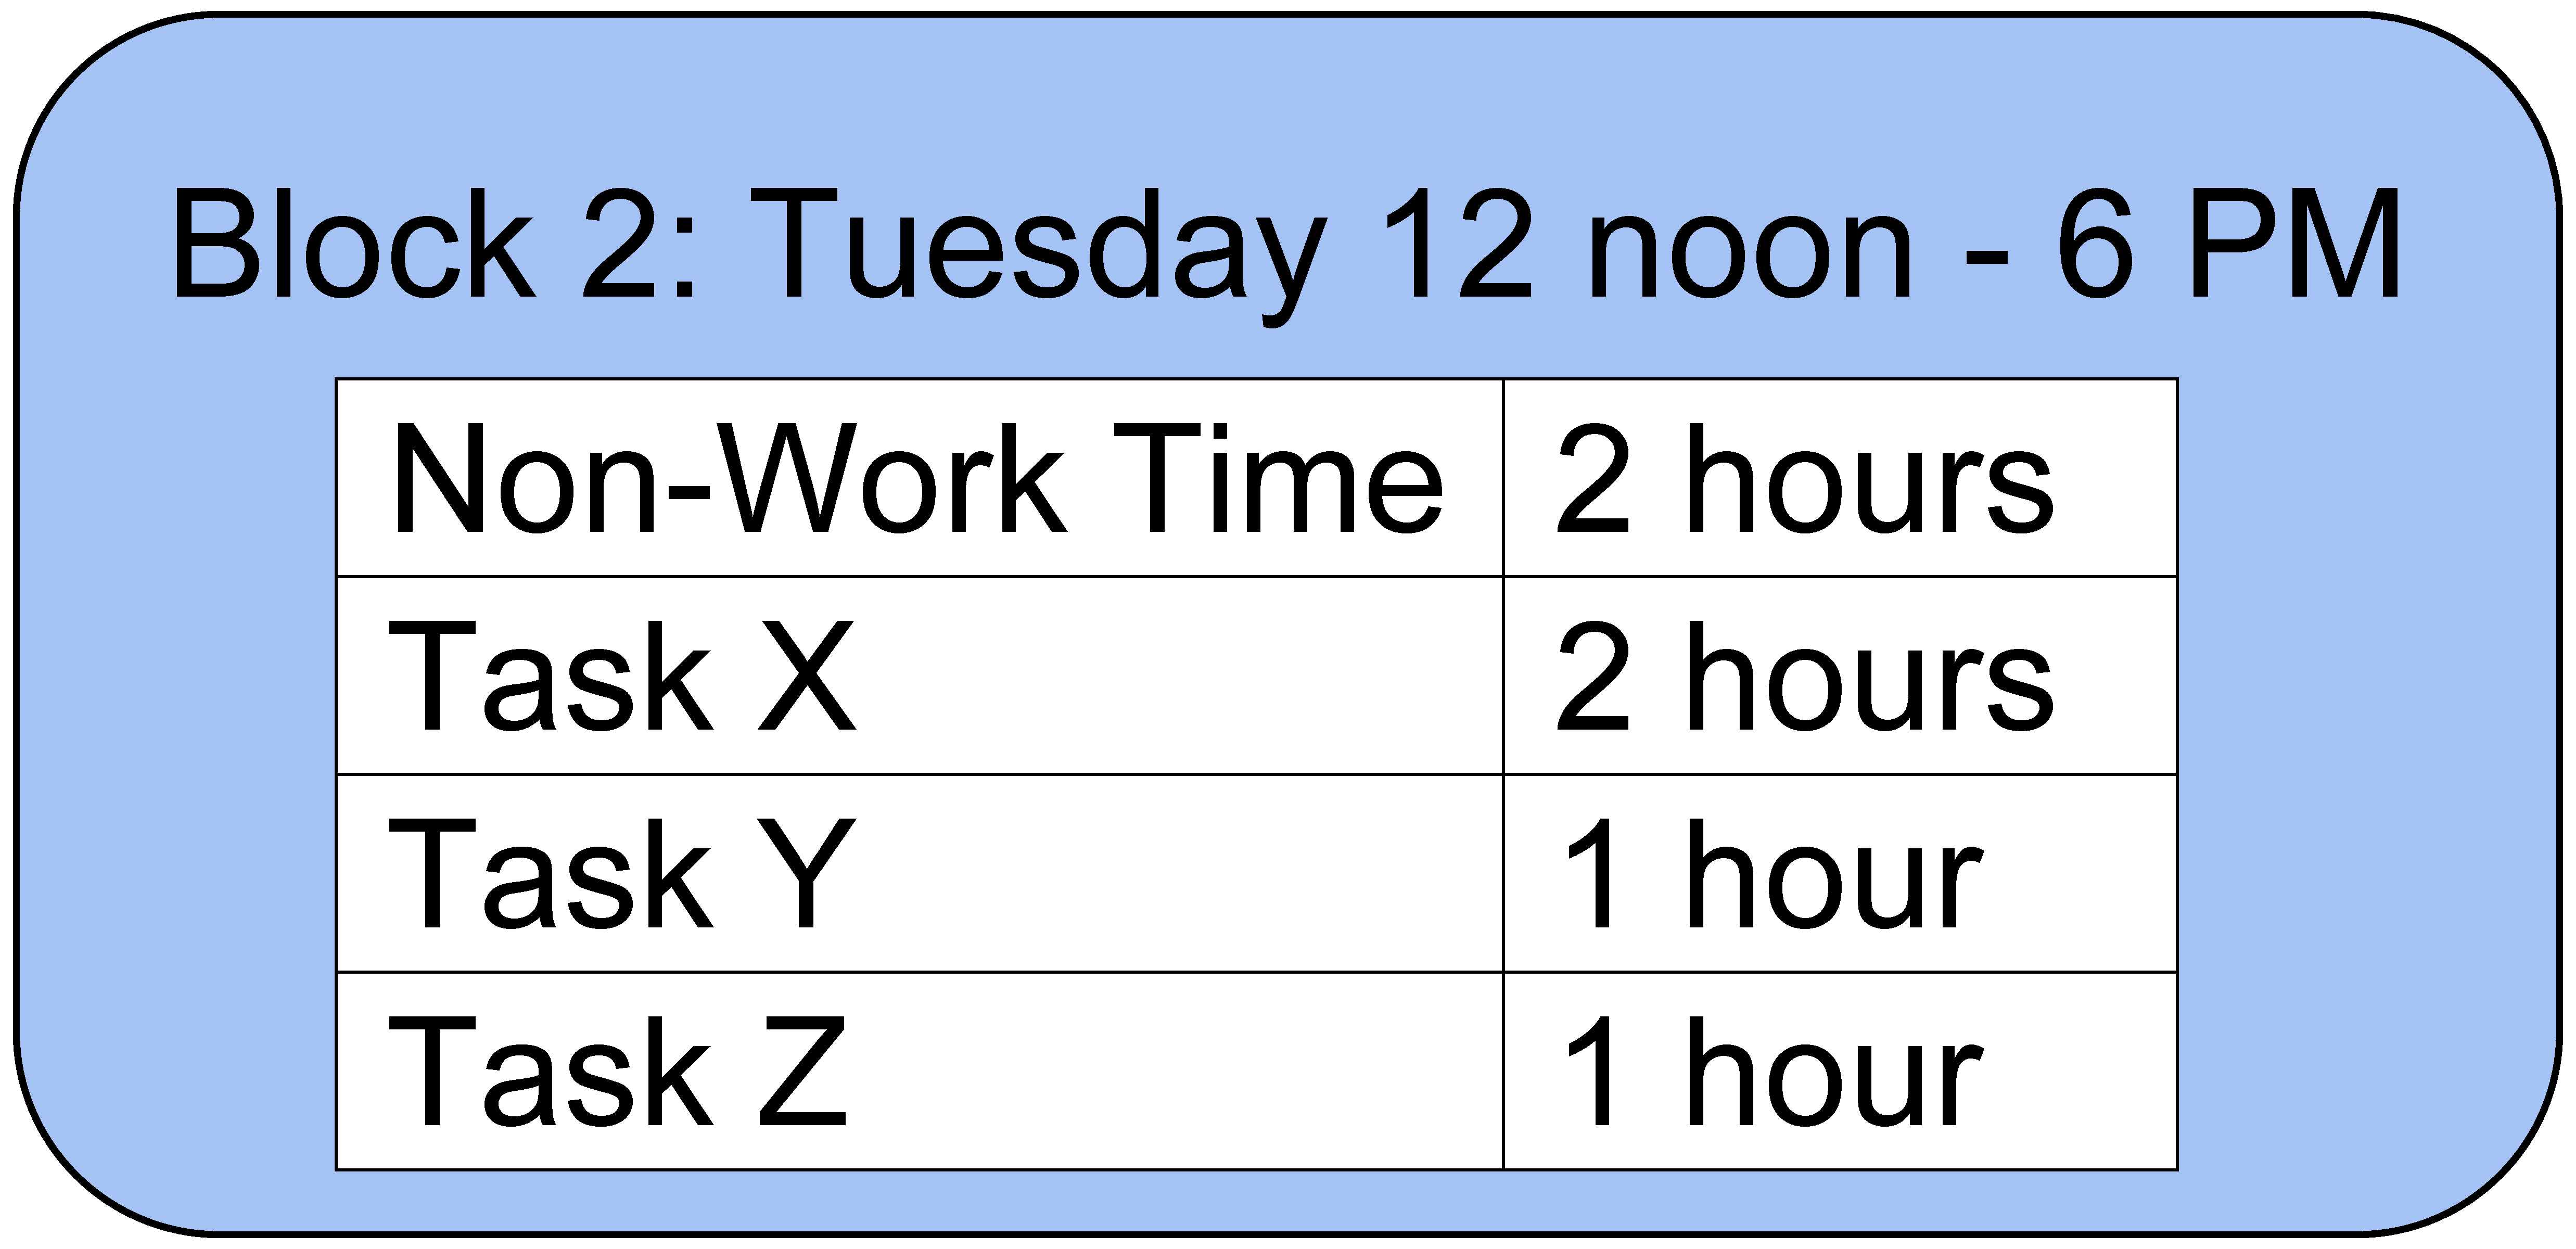
\includegraphics[width=0.48\columnwidth]{Block.pdf}
%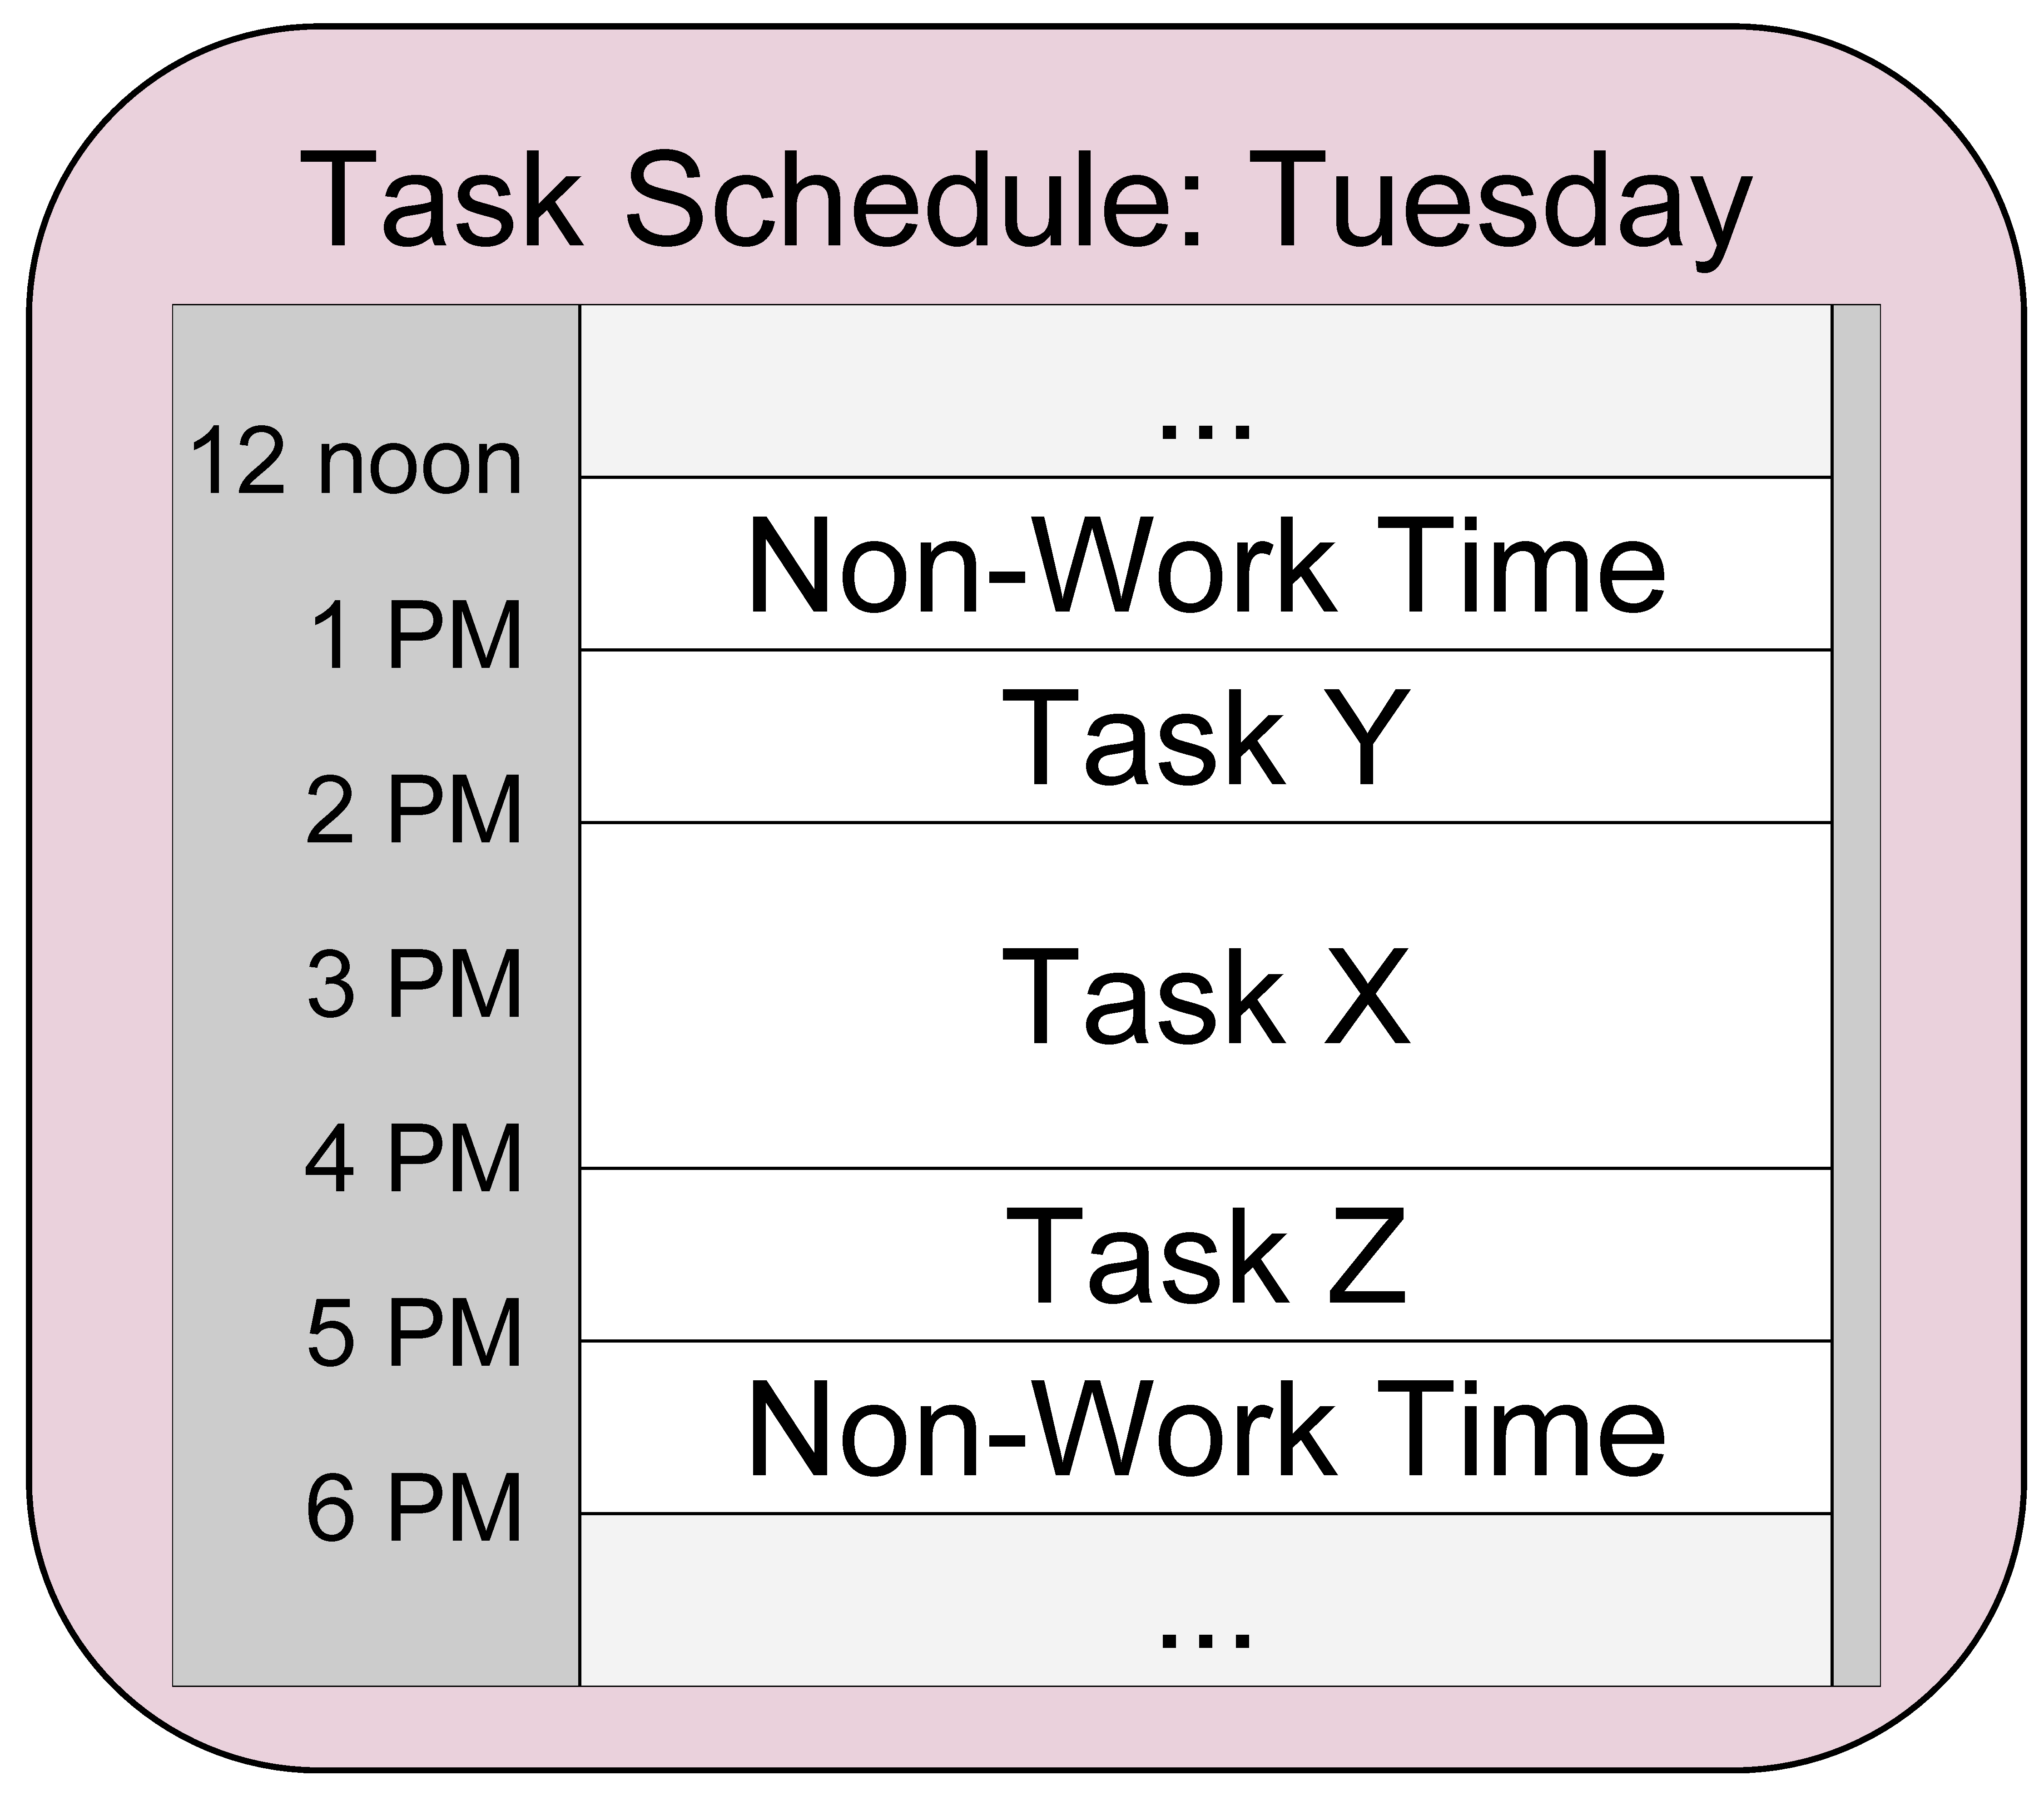
\includegraphics[width=0.48\columnwidth]{Schedule.pdf}

\begin{figure}
  \centering
        \subfloat[][Start with a list of tasks that need to be completed.]{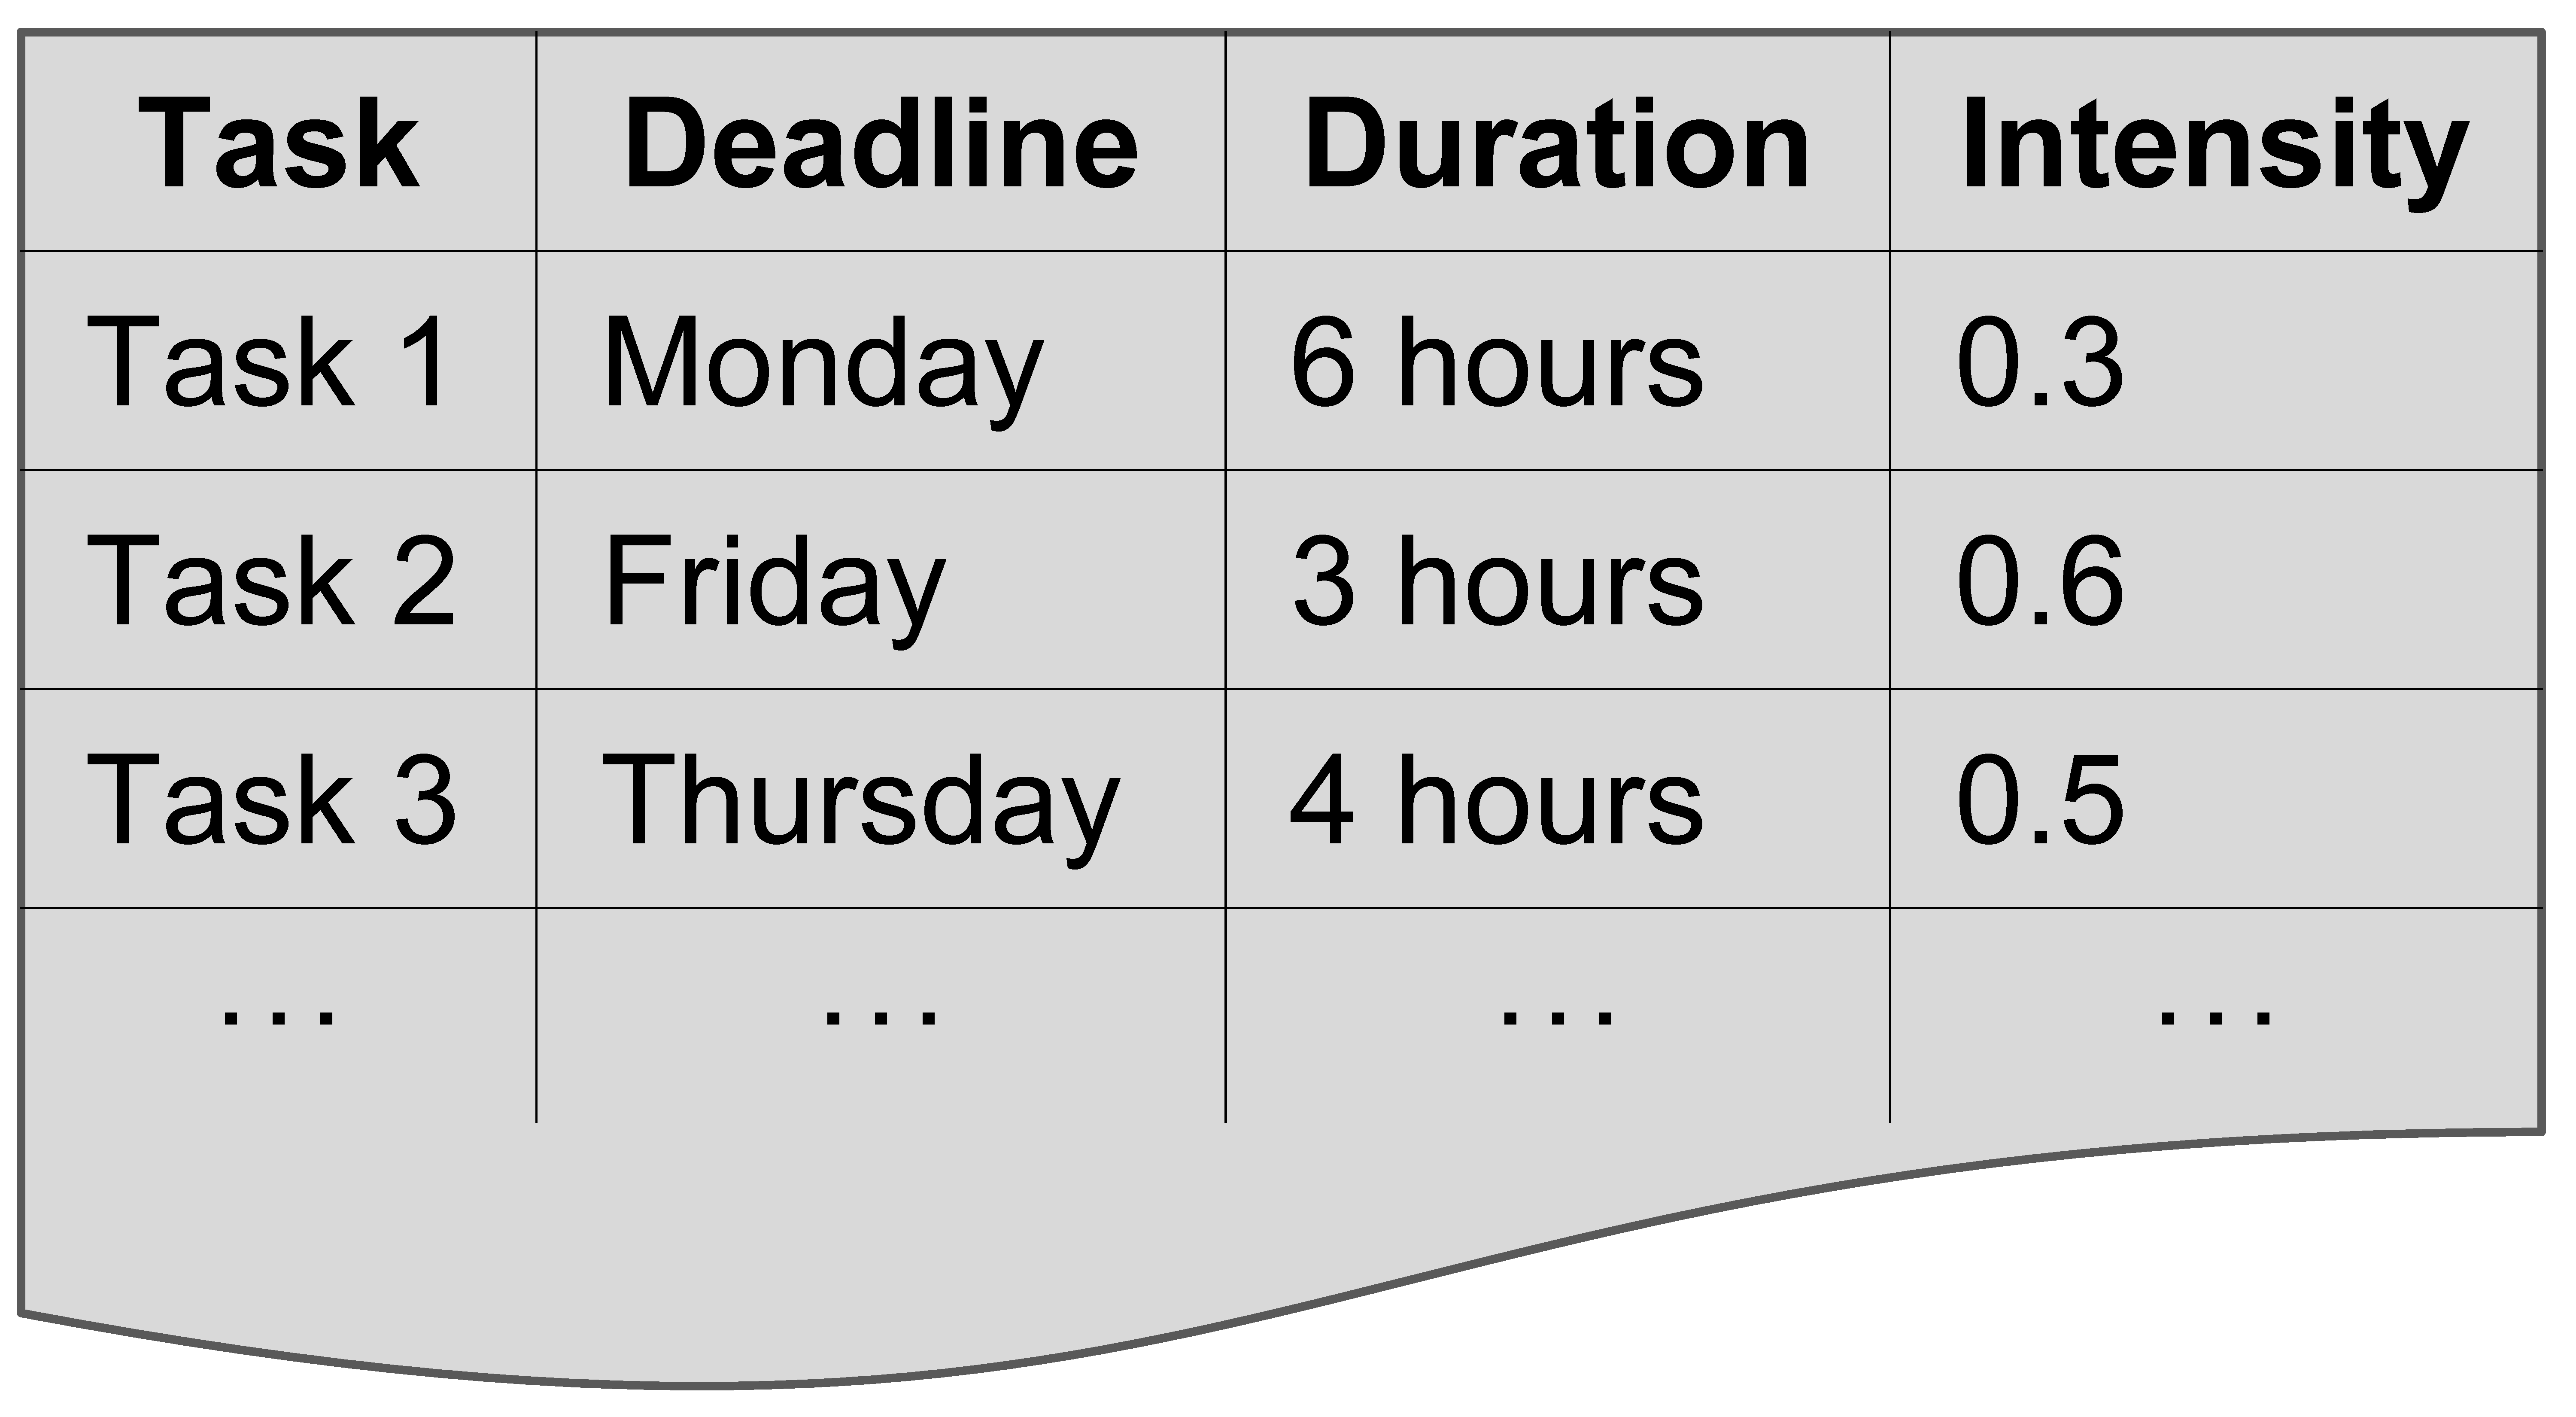
\includegraphics[scale=0.18]{TaskList.pdf}%
                \label{fig:small-mults-orig}%
        }\qquad\qquad
        \subfloat[][Create a section made up of time blocks, and assign tasks to the section. Non-work time is treated as a task.]{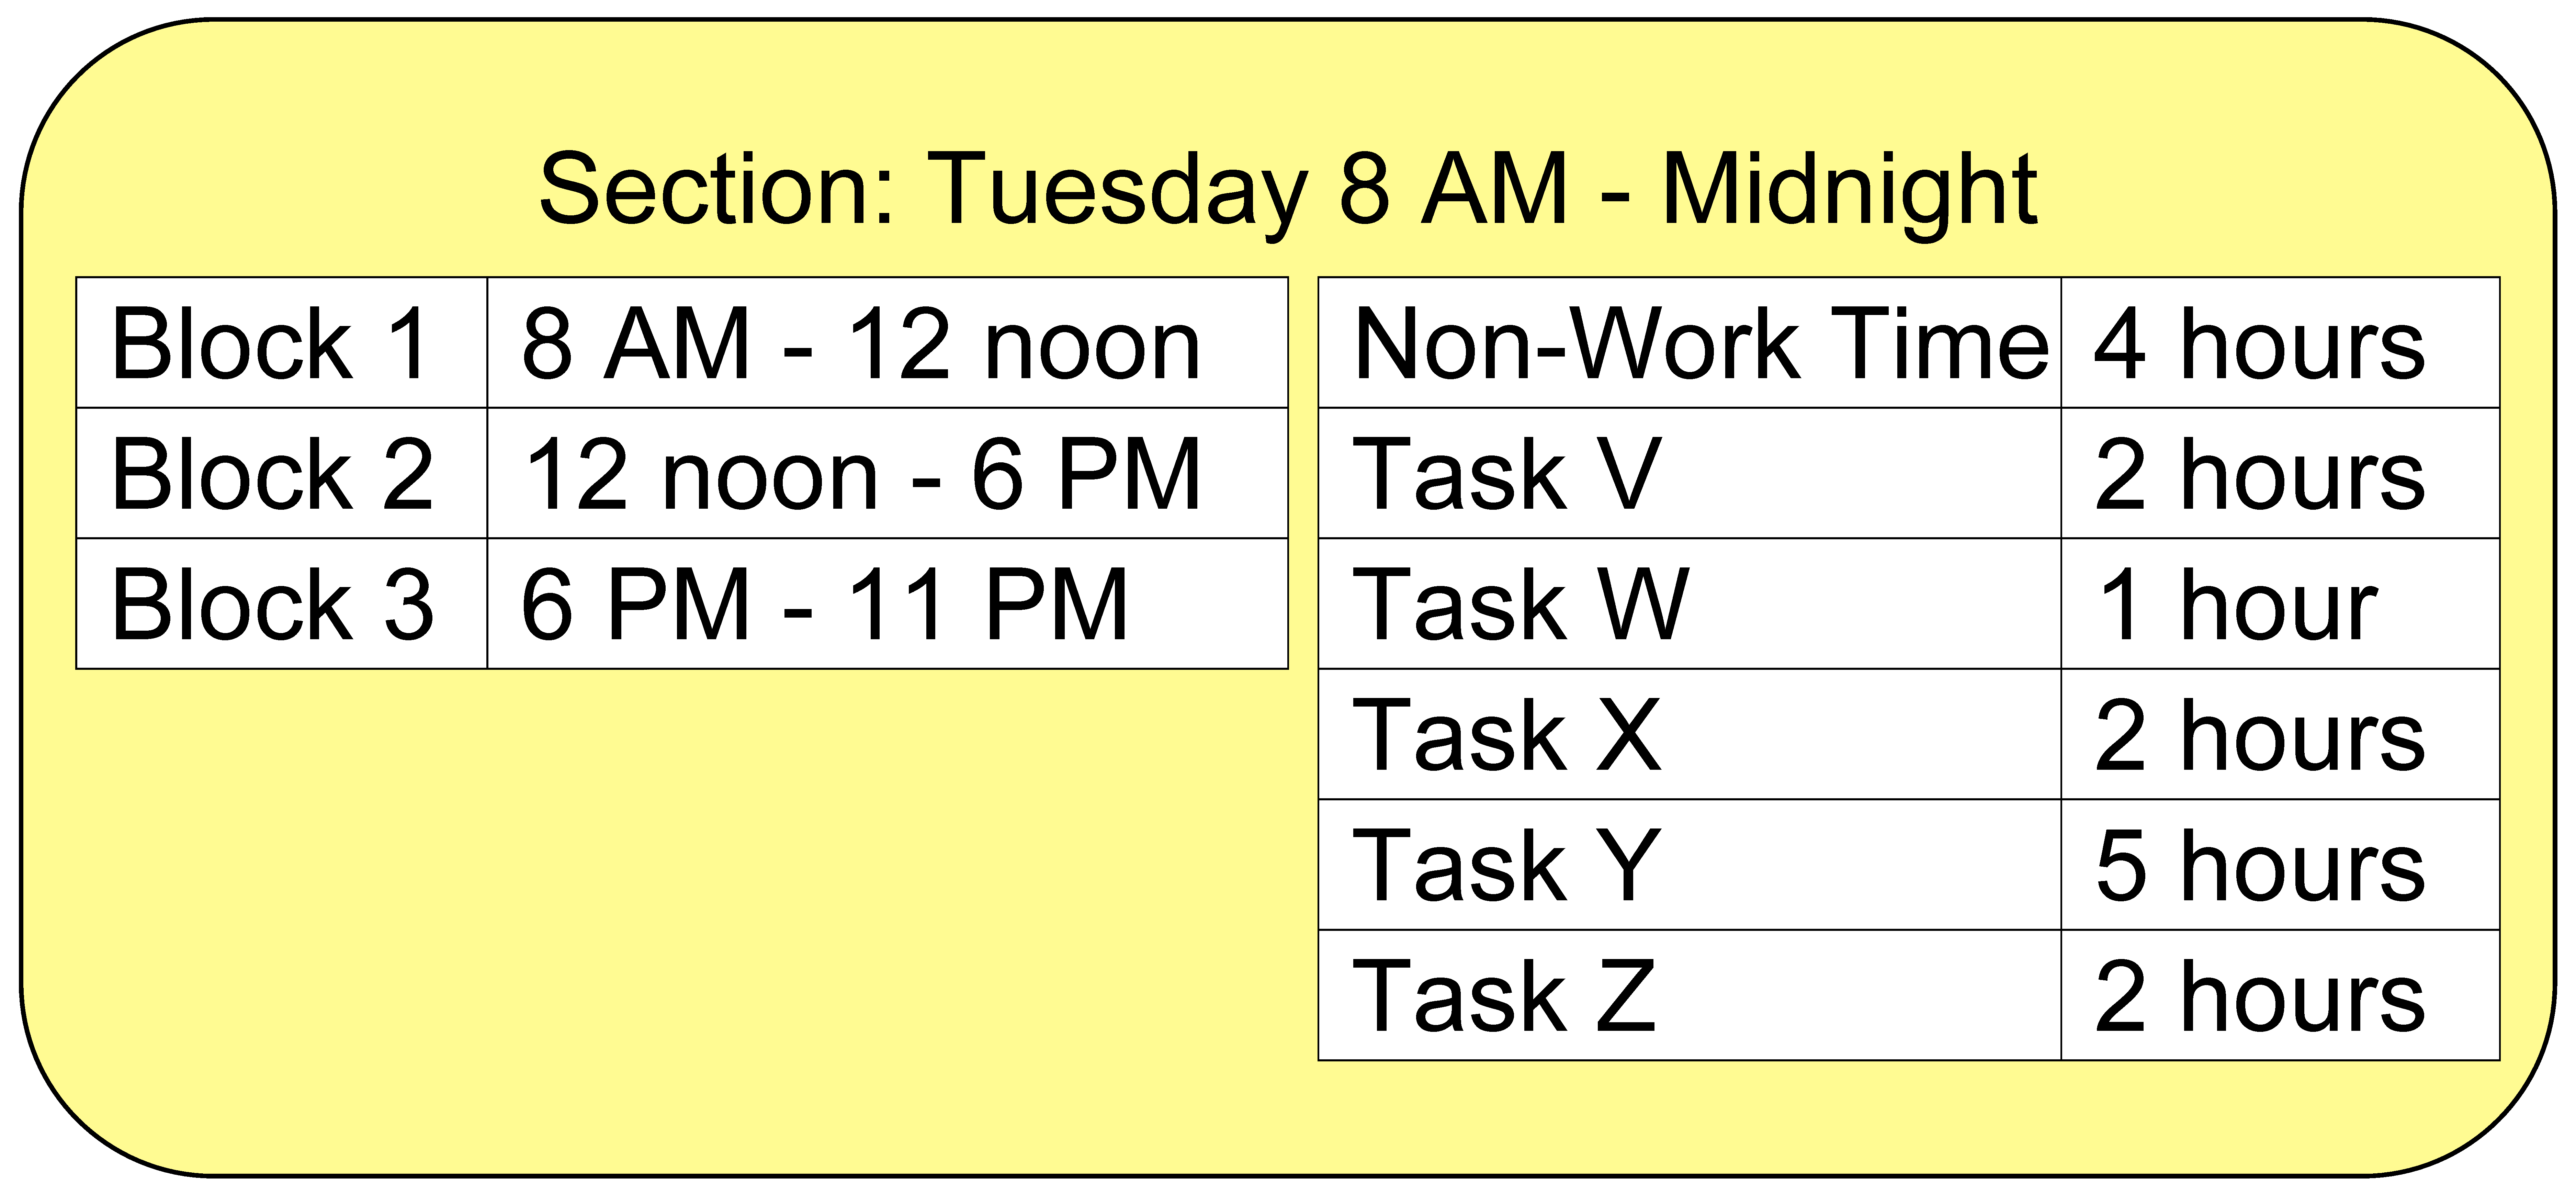
\includegraphics[scale=0.18]{Section.pdf}%
                \label{fig:small-mults-45}%
        }\\
        \subfloat[][Assign tasks to each block in the section.]{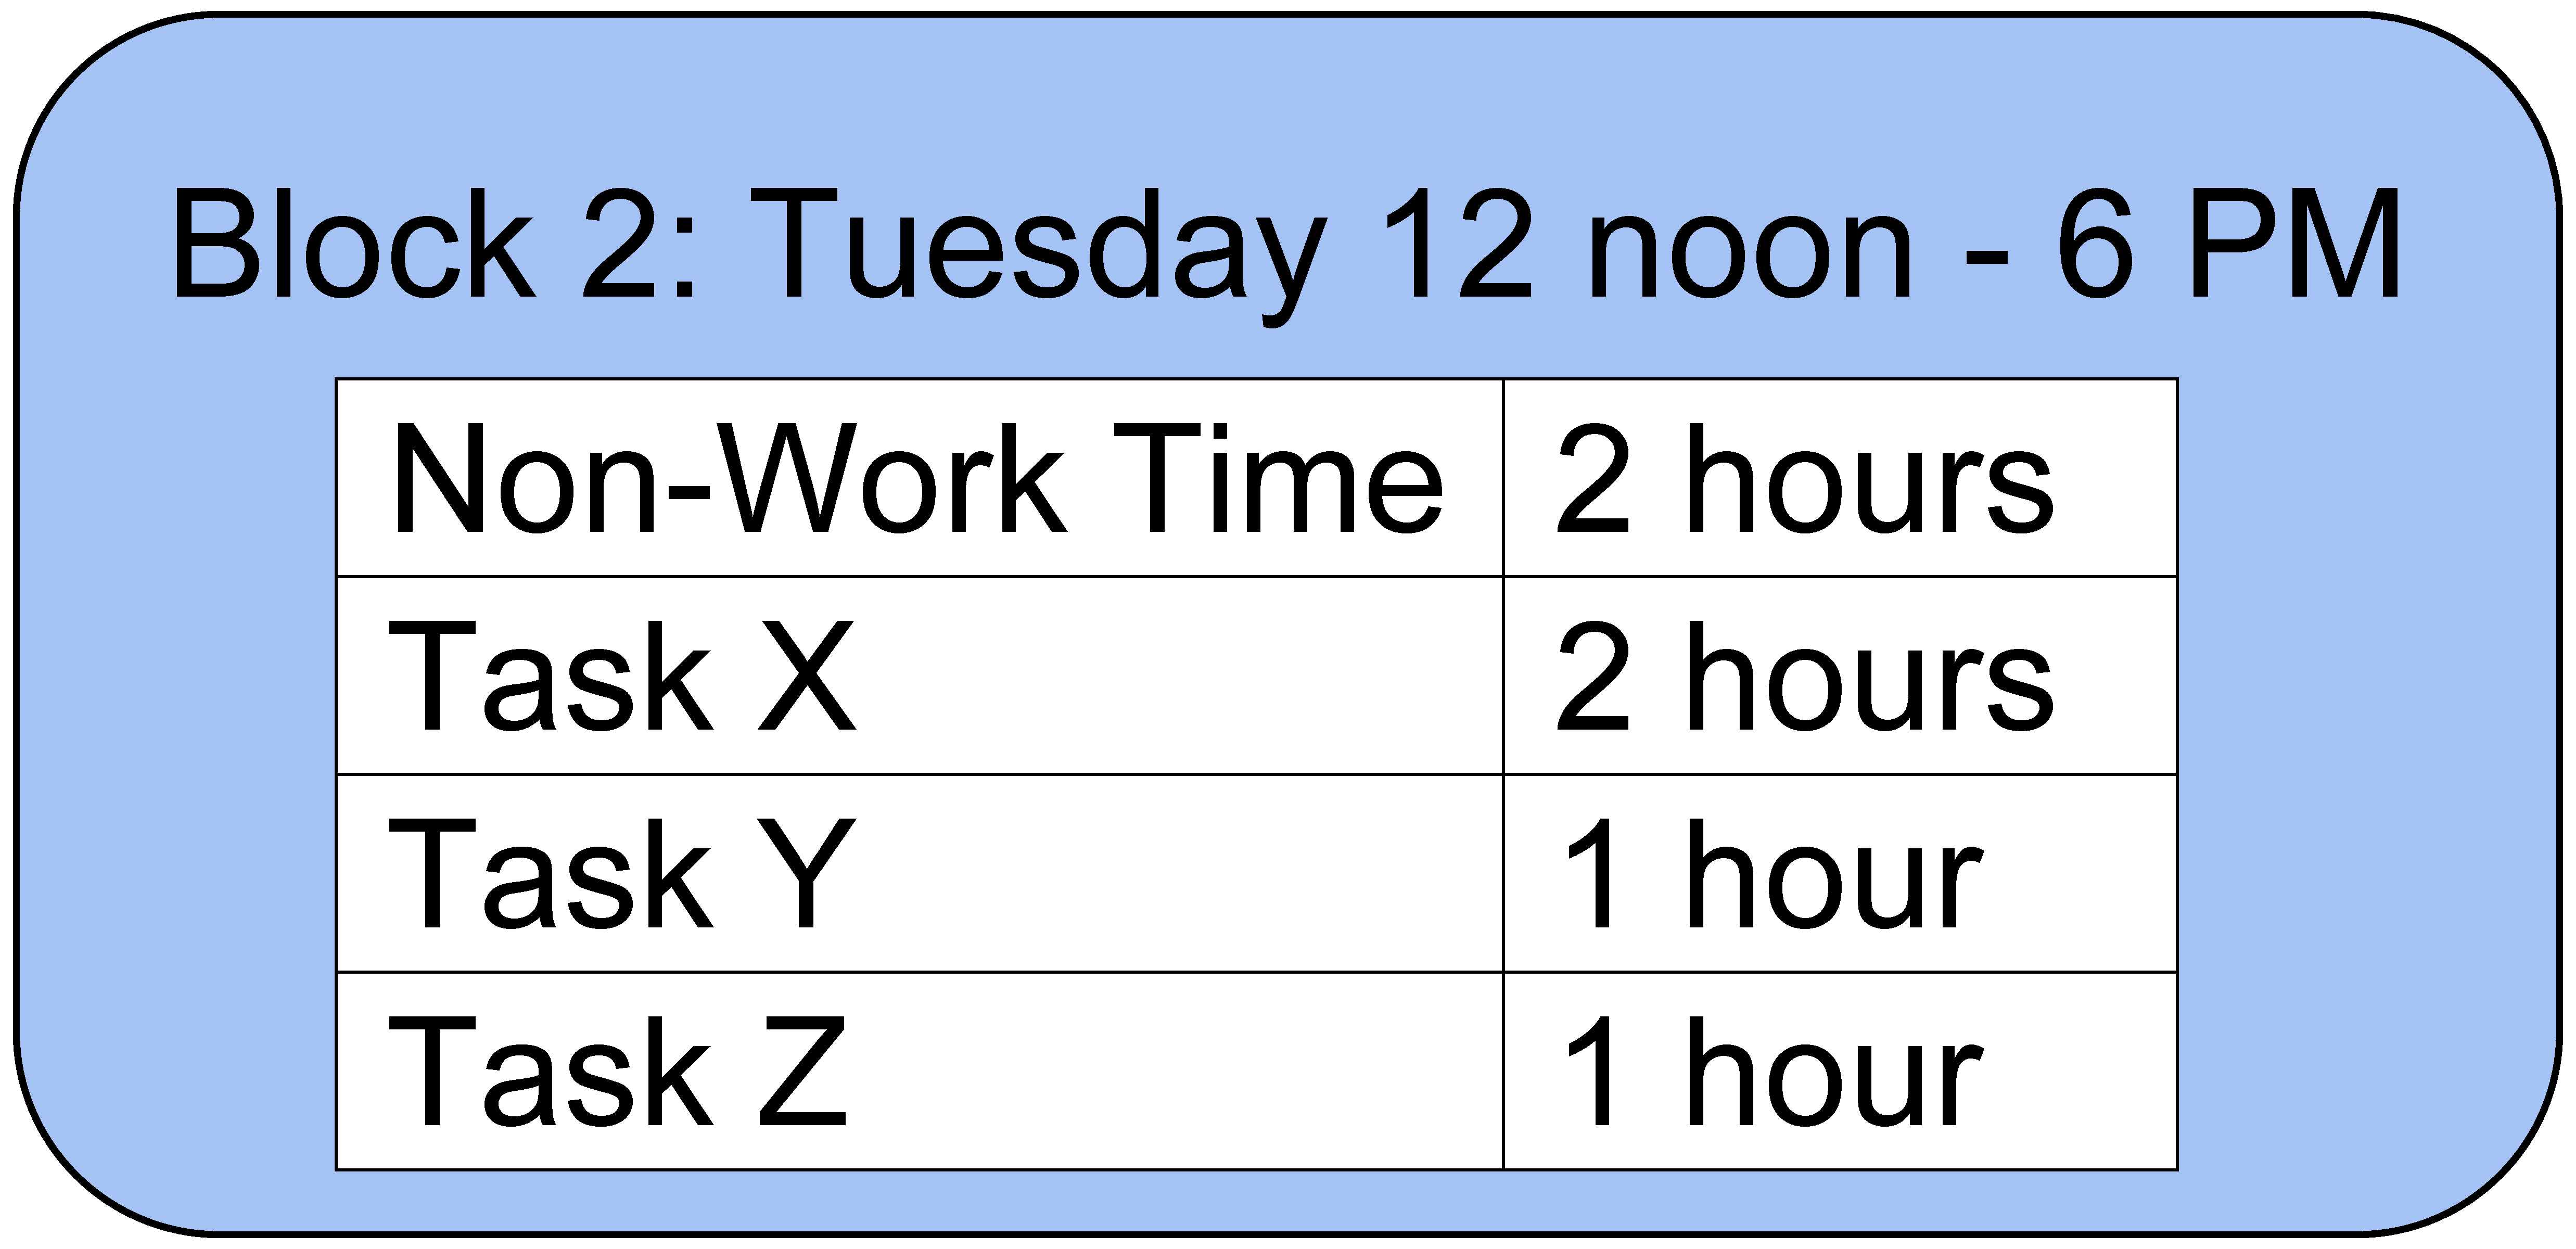
\includegraphics[scale=0.18]{Block.pdf}%
                \label{fig:small-mults-90}%
        }\qquad\qquad
        \subfloat[][Schedule tasks within the block.]{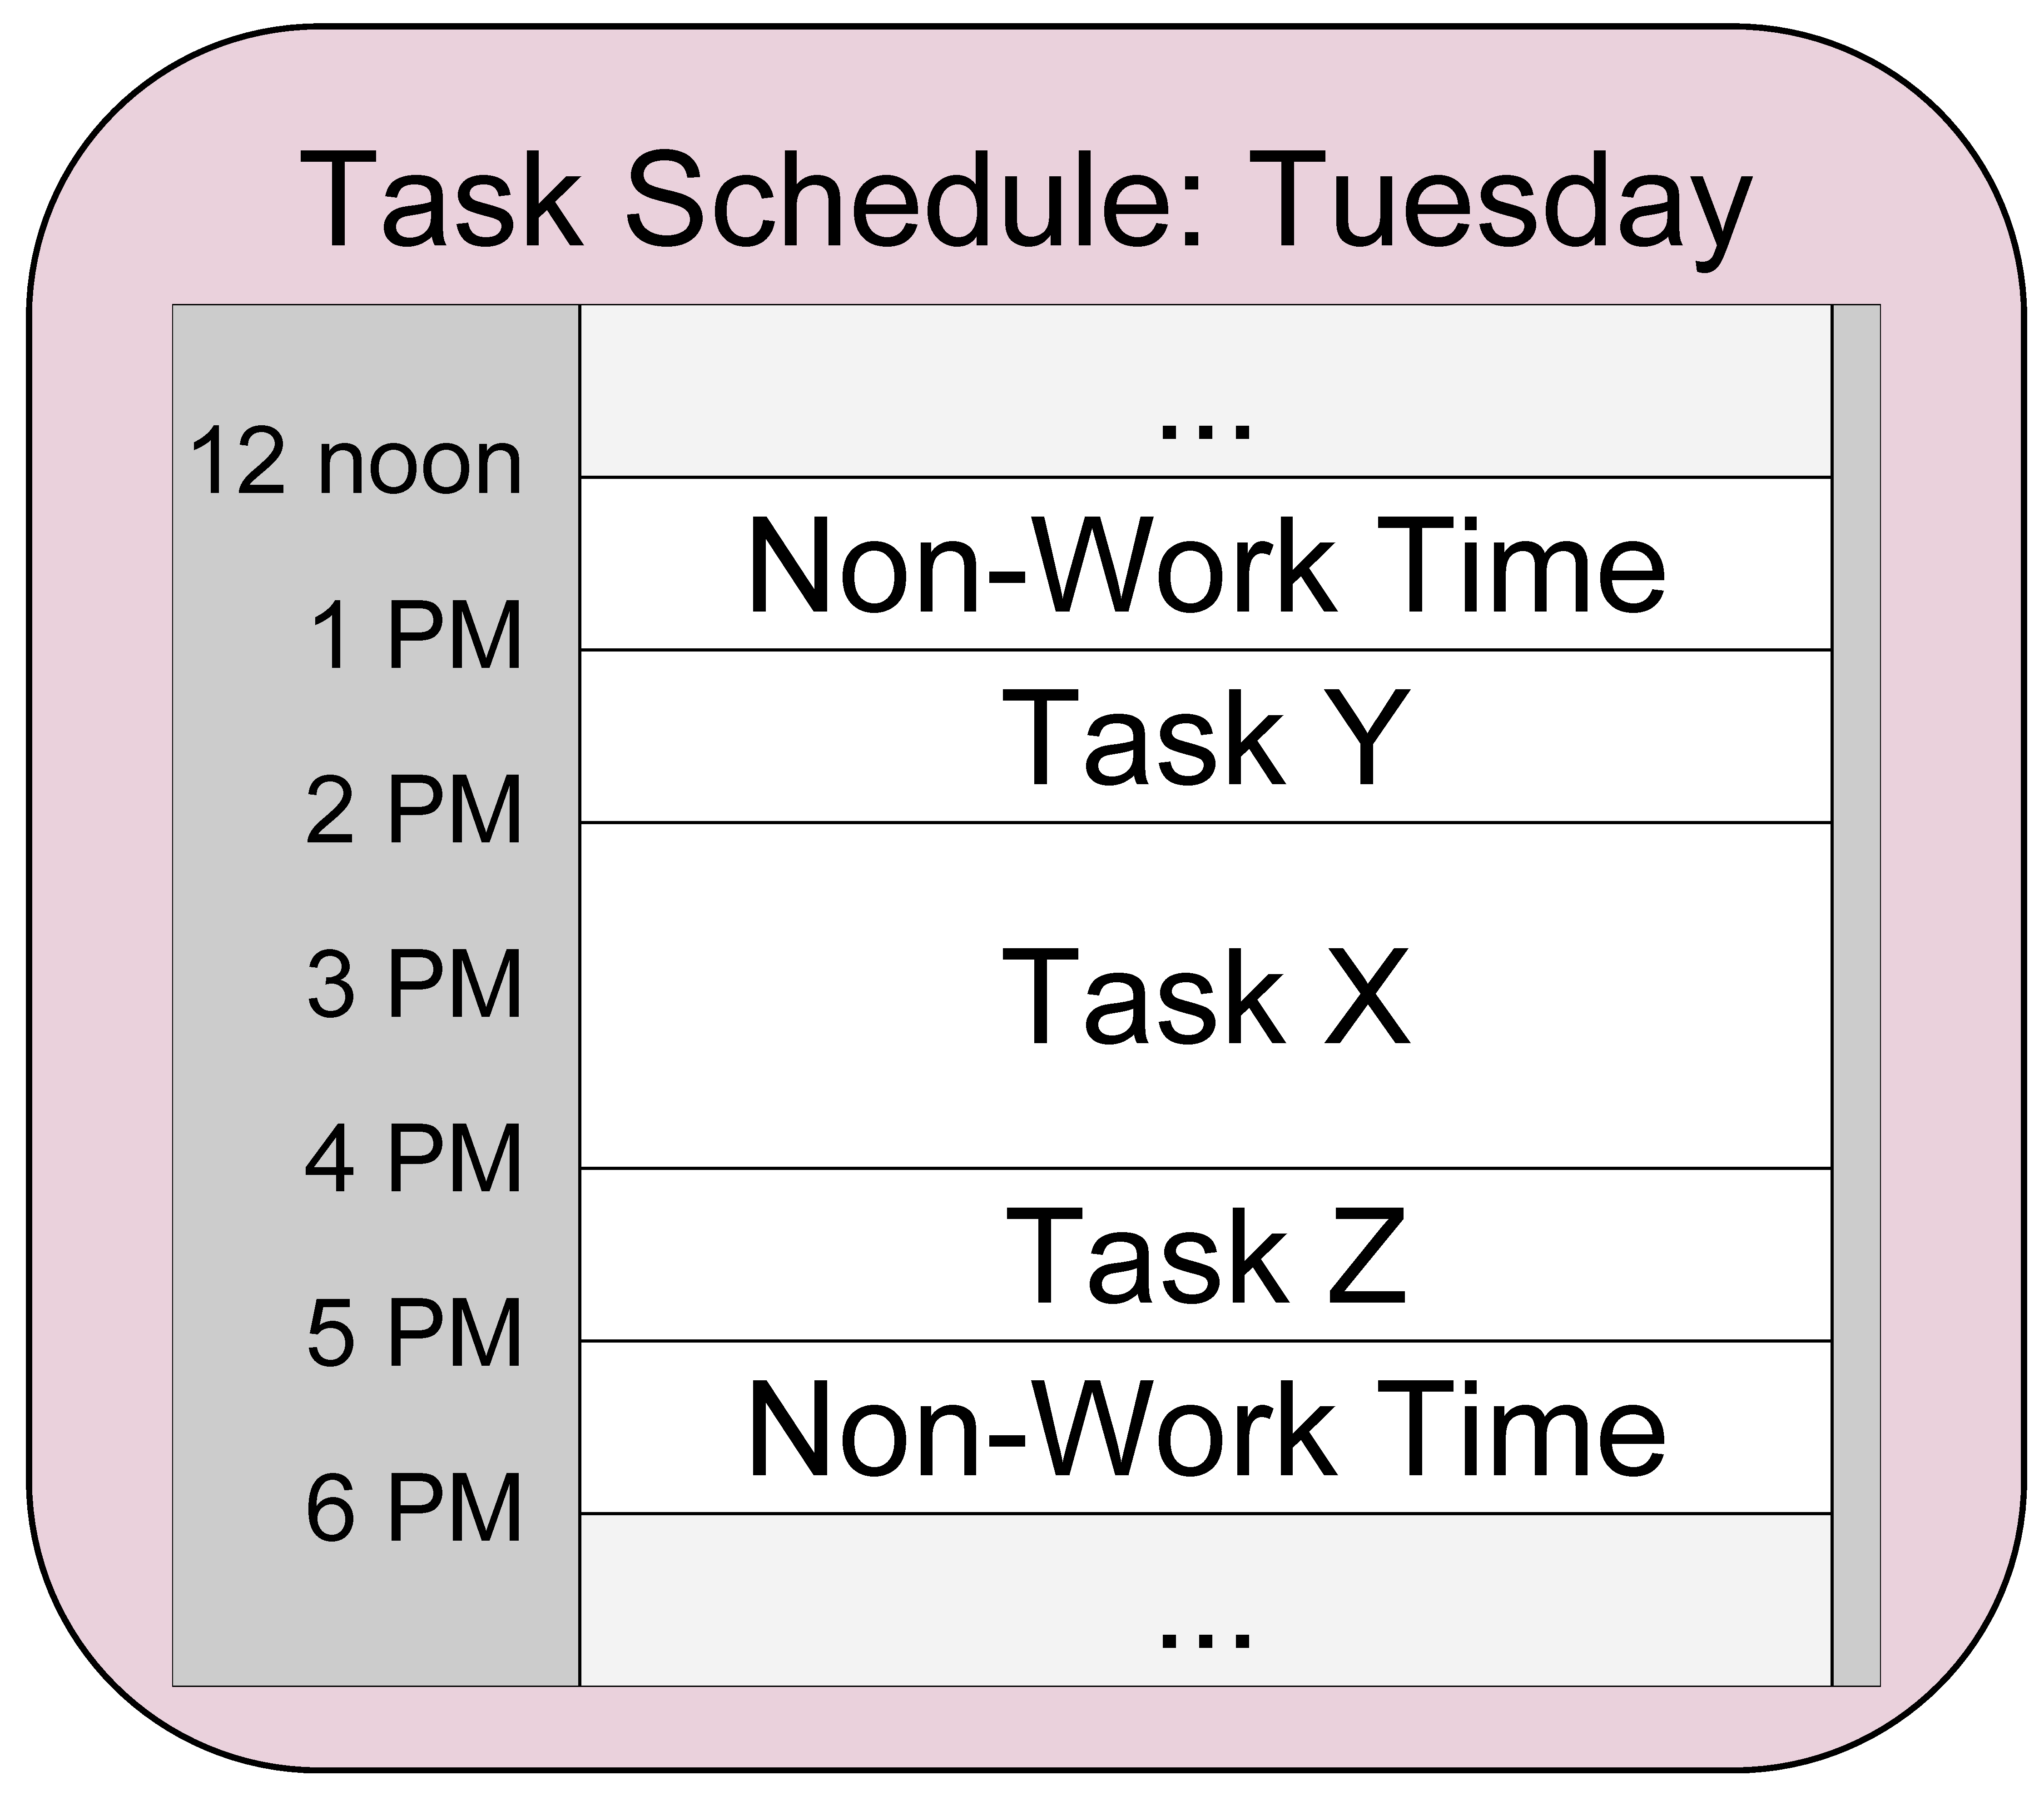
\includegraphics[scale=0.18]{Schedule.pdf}%
                \label{fig:small-mults-135}%
        }
  \caption[Small multiples]{Example for personal scheduling algorithm. Given a task list, assign tasks to sections, then to smaller blocks, then to time slots on the schedule.}%
  \label{fig:small-multiples}
\end{figure}

%\columnbreak


\section{Algorithm for Event Scheduling}
Members of a group often have to schedule events where a number people must attend.
We wanted to create an algorithm capable of scheduling events with multiple attendees.

The event can be either recurring (``regular'') or non-recurring (``special''), has restrictions on available times, some desired or required attendees.
\subsection{Probabilistic Approach}
Using historic data, we can use a probabilistic version of the $k$-nearest neighbors algorithm to determine the likelihoods that all potential attendees will attend a specific event if it is scheduled at some potential times (Holmes).
By summing these likelihoods across all attendees, we are able to get the expected value for the number of people at the event.

\subsection{TODO Title (Approach 2)}
This approach make use of the Personal Scheduling algorithm detailed to the left with some slight modifications.

\section{Future Work}
To further validate this work, it will be useful to test the algorithms on actual scheduling problems.
For the personal scheduling algorithm, it will be helpful to collect schedule data from individuals who are interested in applying the algorithm to their own schedules. Their feedback can be used to evaluate and revise the algorithm to better suit their needs preferences.
For event scheduling, data would need to be collected from an organization, preferably one that is willing to use the algorithm to schedule their events.
Additionally, for an organization that uses a common calendar application, it would be interesting to integrate the event scheduling algorithms with the calendar to automatically schedule events.



\section{References}
\bibliographystyle{hmcmath}
%\bibliography{sampleposter}
C.~C.~Holmes and N.~M.~Adams. \emph{A probabilistic nearest neighbour method for statistical pattern recognition} (2002). \url{http://hedibert.org/wp-content/uploads/2016/02/holmes-adams-2002.pdf}


\section{For Further Information}
For more information about this project, please contact \url{sbost@hmc.edu} or \url{gu@hmc.edu}.


\section{Acknowledgments}
I would like to thank Professor Weiqing Gu for her guidance throughout this research.
I am also very grateful to the Rose	Hills	Foundation Science \& Engineering Summer Undergraduate Research Fellowship program for their kind and generous support of this project.


\end{poster}

\end{document}

 
